\newpage
\section{$\Hbb$ tagger limits (categories Hbb1, Hbb2)}
\label{results}

\iffalse

\begin{figure*}[h!tpb]
\begin{center}
\includegraphics[width=0.70\textwidth]{trunk/brazilianFlag_HbbWqqHPLP.pdf}
\includegraphics[width=0.49\textwidth]{}
\includegraphics[width=0.49\textwidth]{}
\end{center}
\caption{Expected and observed limits for H(bb)Z(qq) search. The combined limit is on top. 
The high purity is on the bottom left. the low purity V-tagging on bottom right.   
%  The predicted cross sections as a function of resonance mass for the considered benchmark models are overlaid.
}
\label{fig:HbbZqqLimits}
\end{figure*}

\begin{figure*}[h!tpb]
\begin{center}
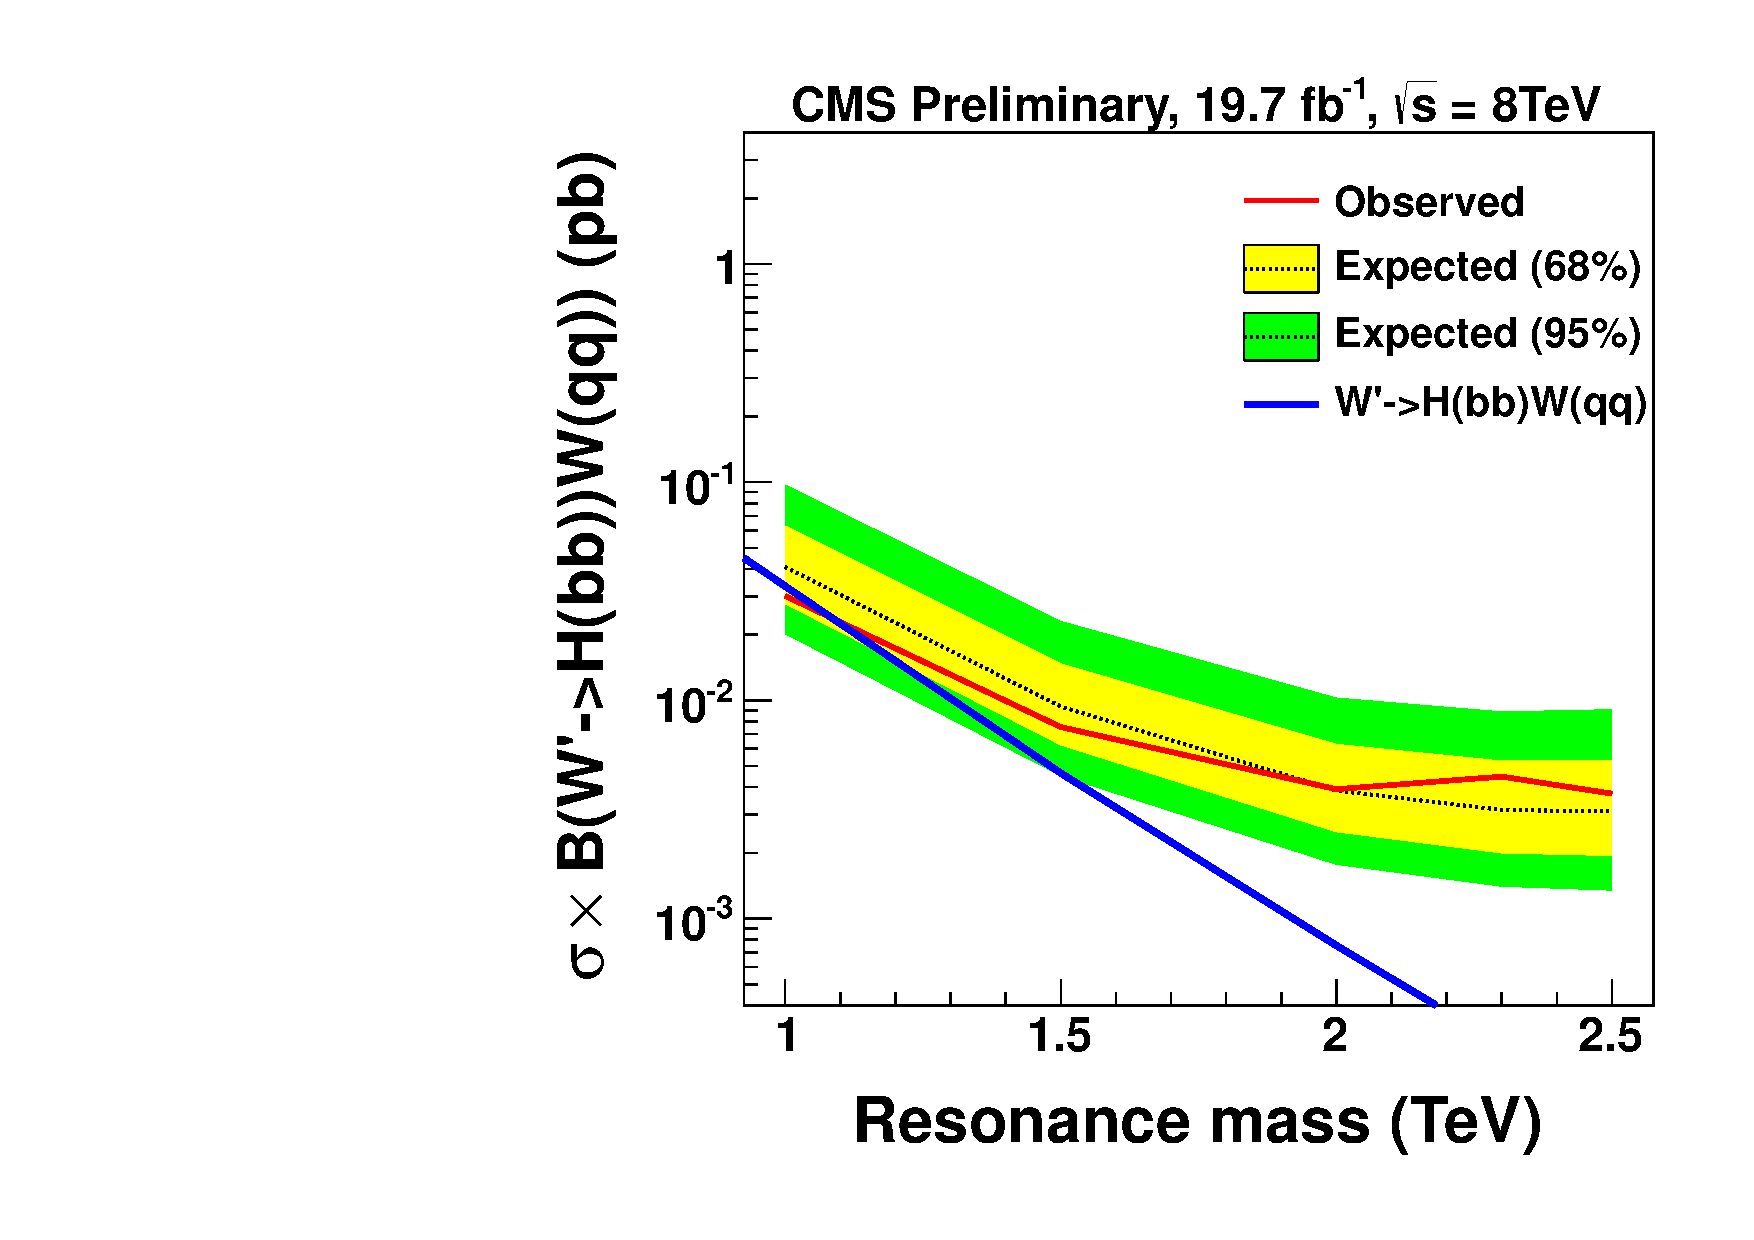
\includegraphics[width=0.70\textwidth]{HbbZqqfigs/Limits/brazilianFlag_Hbb_HbbWqqCombine.pdf}
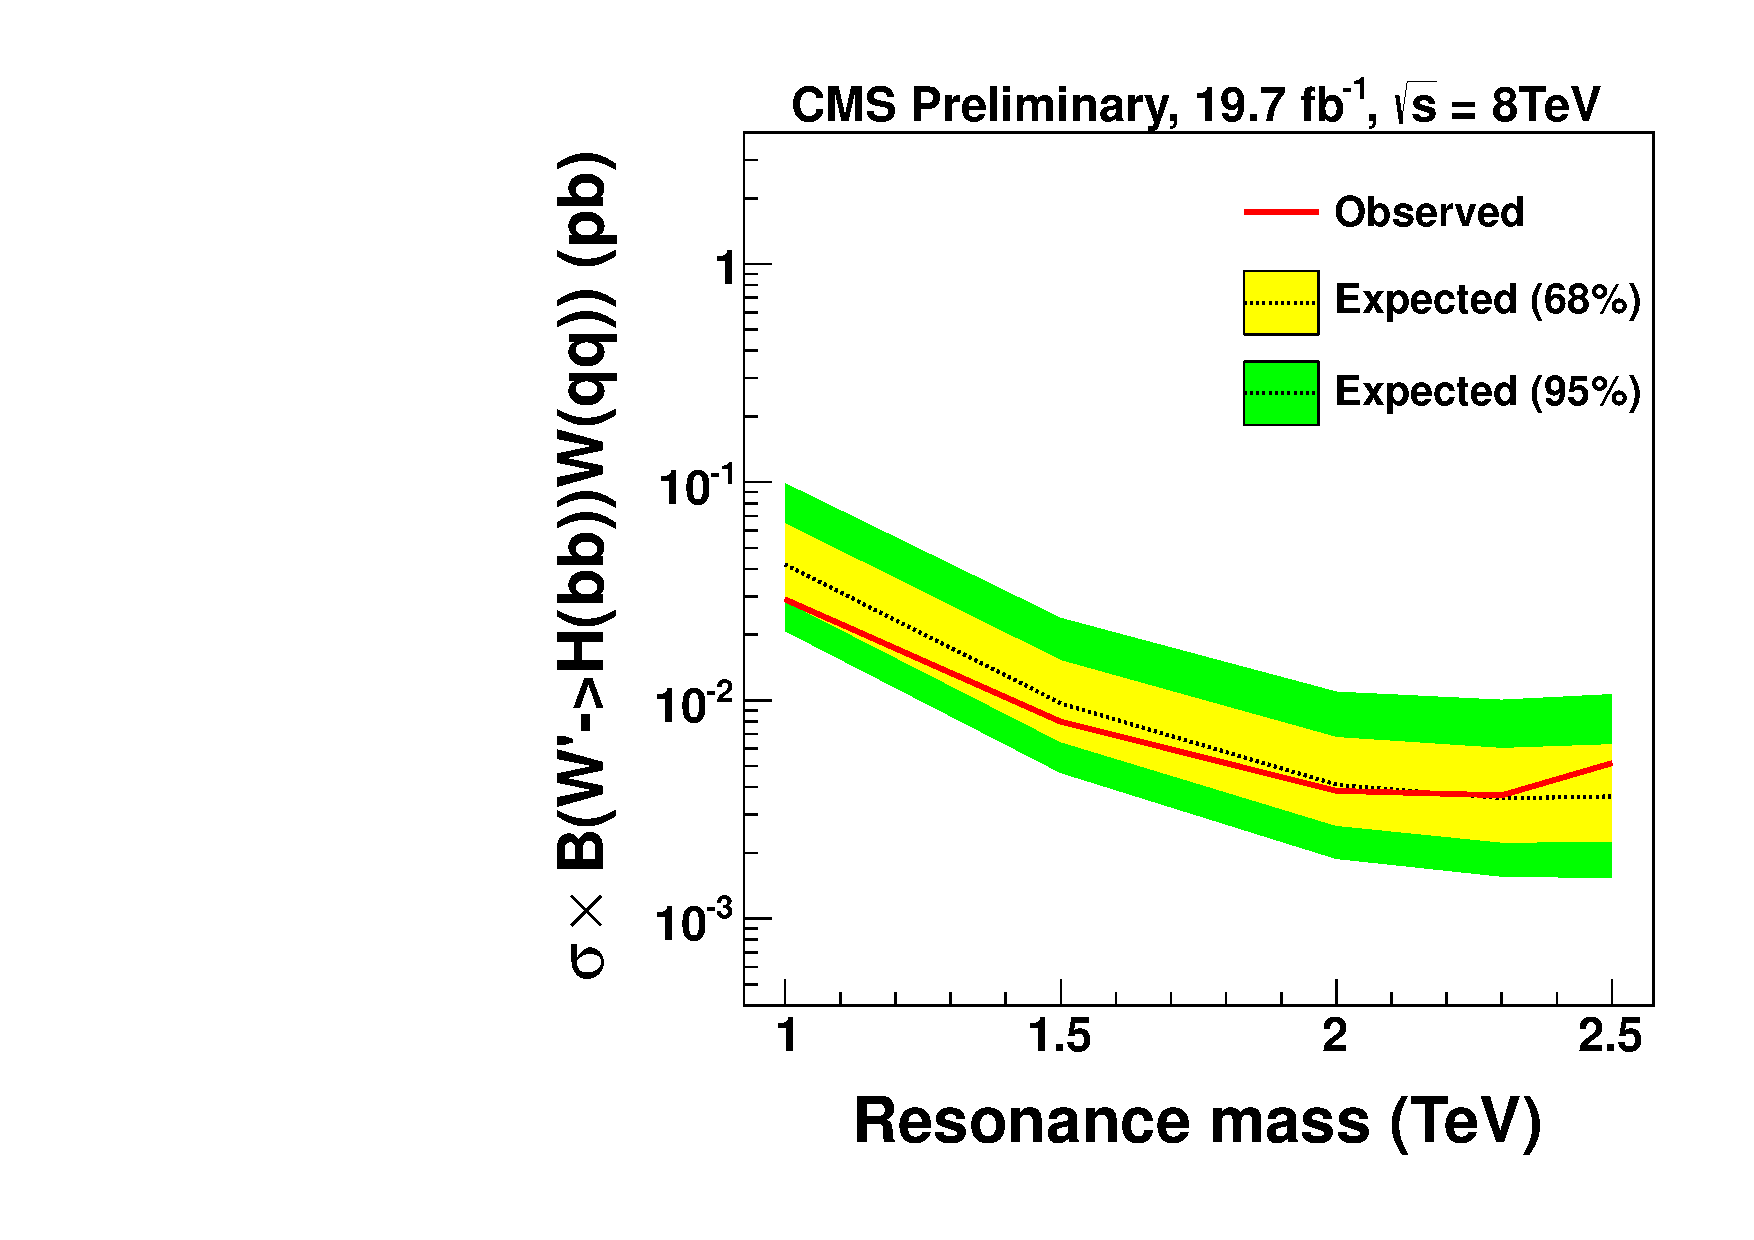
\includegraphics[width=0.49\textwidth]{HbbZqqfigs/Limits/brazilianFlag_Hbb_HbbWqqHighP.pdf}
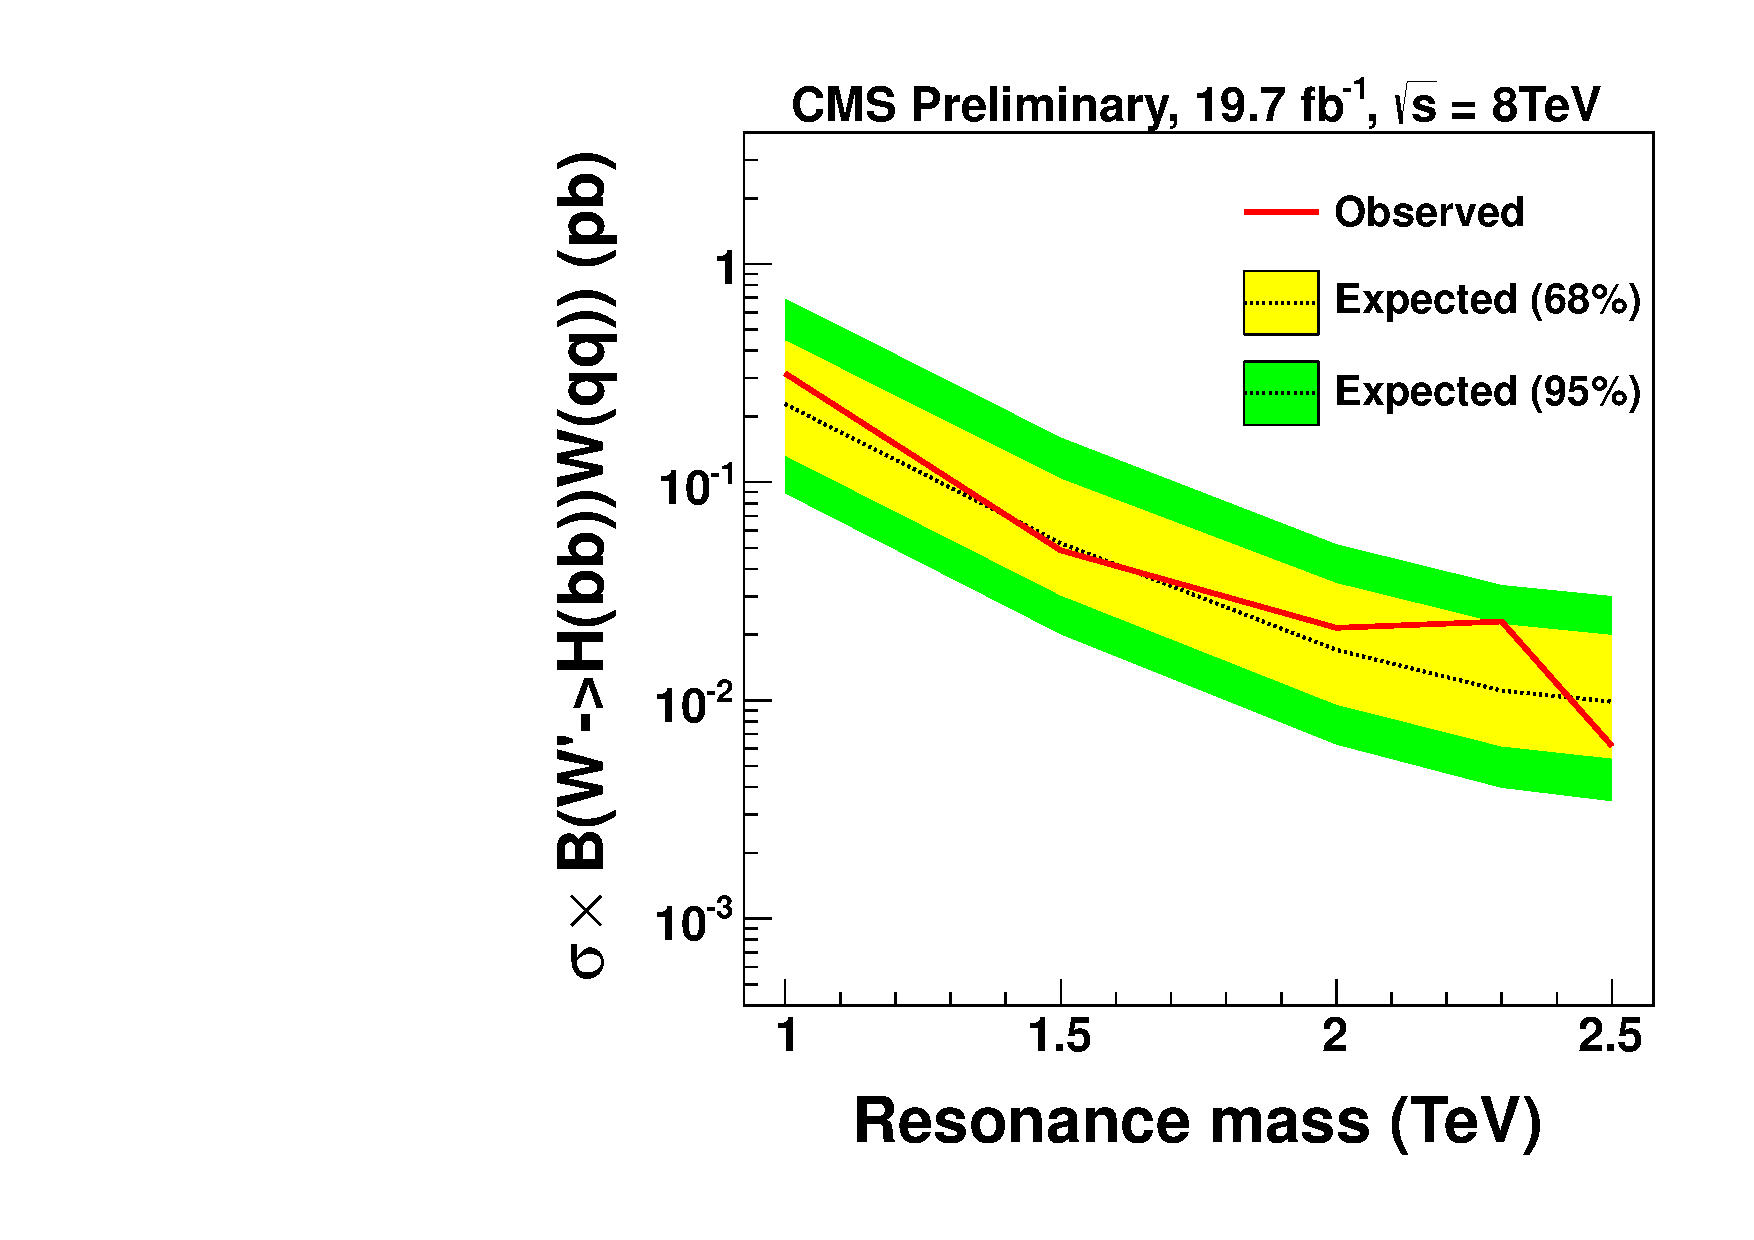
\includegraphics[width=0.49\textwidth]{HbbZqqfigs/Limits/brazilianFlag_Hbb_HbbWqqLowP.pdf}
\end{center}
\caption{Expected and observed limits for H(bb)W(qq) search. The combined limit is on top.
The high purity is on the bottom left. the low purity V-tagging on bottom right.
%  The predicted cross sections as a function of resonance mass for the considered benchmark models are overlaid.
}
\label{fig:HbbWqqLimits}
\end{figure*}

\fi

Figure~\ref{fig:HbbVCombined} shows the limits for \HbbVqq signals passing the 
$\Hbb$ tagger. Limits of combining catogories Hbb1 and Hbb2 are presented. 
The $\Hbb$ and V bosons braching ratios are already taken into account.


\begin{figure*}[ht!pb]
\begin{center}
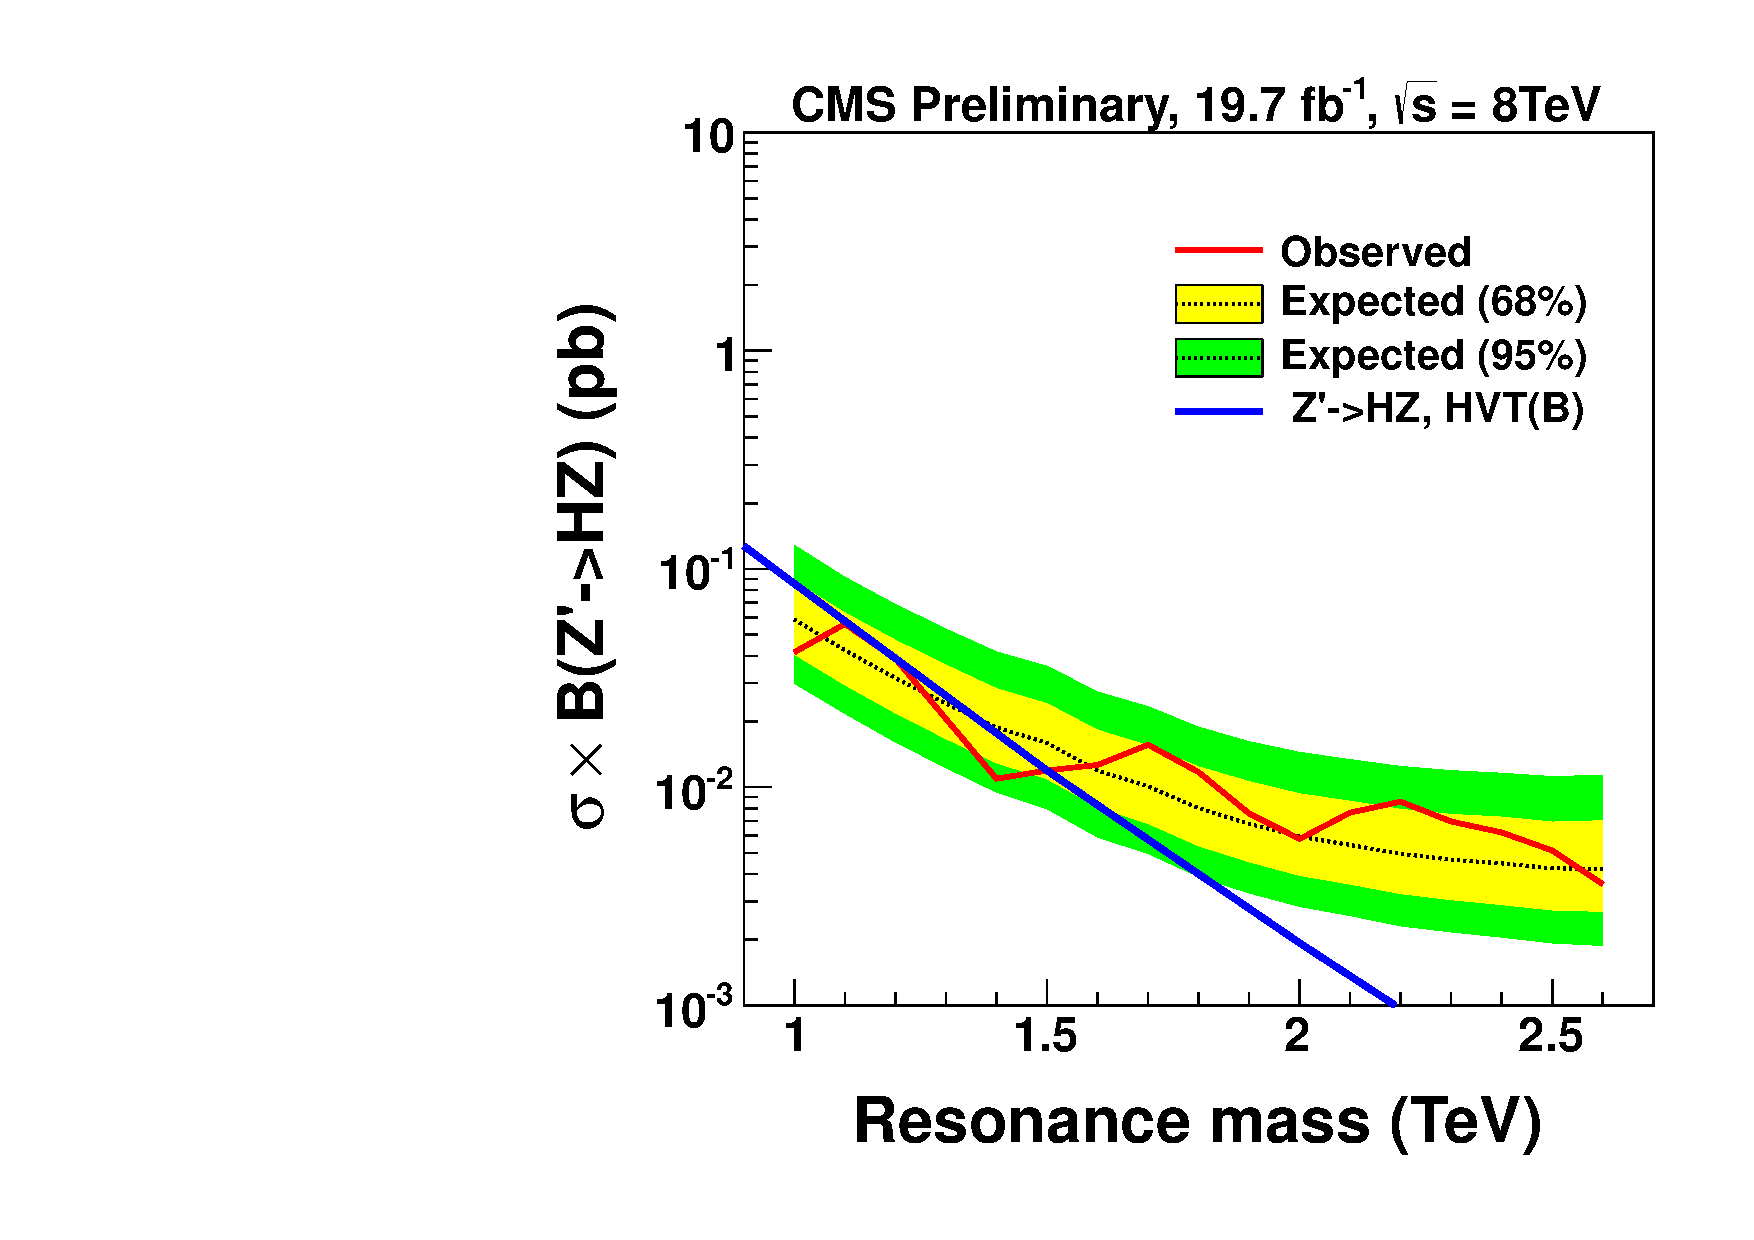
\includegraphics[width=0.49\textwidth]{brazilianFlag_HbbZqqHPLP.pdf}
\includegraphics[width=0.49\textwidth]{brazilianFlag_HbbWqqHPLP.pdf}
\end{center}
\caption{Expected and observed limits for ${\rm Z'\to HZ}$(left) and ${\rm W' \to WZ}$(right)
 search, in $\Hbb$ decay mode. Branching ratios of $\Hbb$ and V decays are
 taken into account.Theory model used here is HVT scenario B, arXiv:1402.4431.
% The high purity is on the bottom left. the low purity V-tagging on bottom right.
%  The predicted cross sections as a function of resonance mass for the considered benchmark models are overlaid.
}
\label{fig:HbbVCombined}
\end{figure*}



\clearpage
